\chapter{McCabe's Cyclomatic Complexity}
McCabe's cyclomatic complexity (CC) is a software quality metric that quantifies the complexity of a software program. Complexity is inferred by measuring the number of linearly independent paths through the program. The higher the number the more complex the code.\todo{A little bit more explanation is needed.}
The basis of CC calculation is the \emph{control flow graph} \autocite{spillner2021software}.

\section{From Cyclomatic Complexity to Unit Tests}
To calculate CC, a flow graph is utilized to depict control flow. Each node in the graph indicates several statements in the program and the flow of control is represented by directed edges. An example for such a graph is given in Figure \ref{fig:flow-graph-eg} for the code shown in Listing \ref{lst:pos_sum}.

\begin{lstlisting}[caption={pos\_sum finds the sum of all positive numbers stored in an integer array a. Input parameter is a, an array of integers. The output of the function is sum, the sum of integers inside the array a.},label=lst:pos_sum]
int pos_sum(int[] a) {
    int sum = 0;
    int i = 0;
    while (i < a.length) {
        if (a[i] >= 0) {
            sum += a[i];
        }
        i++;
    }
    return sum;
}
\end{lstlisting}

\begin{figure}[H]
    \centering
    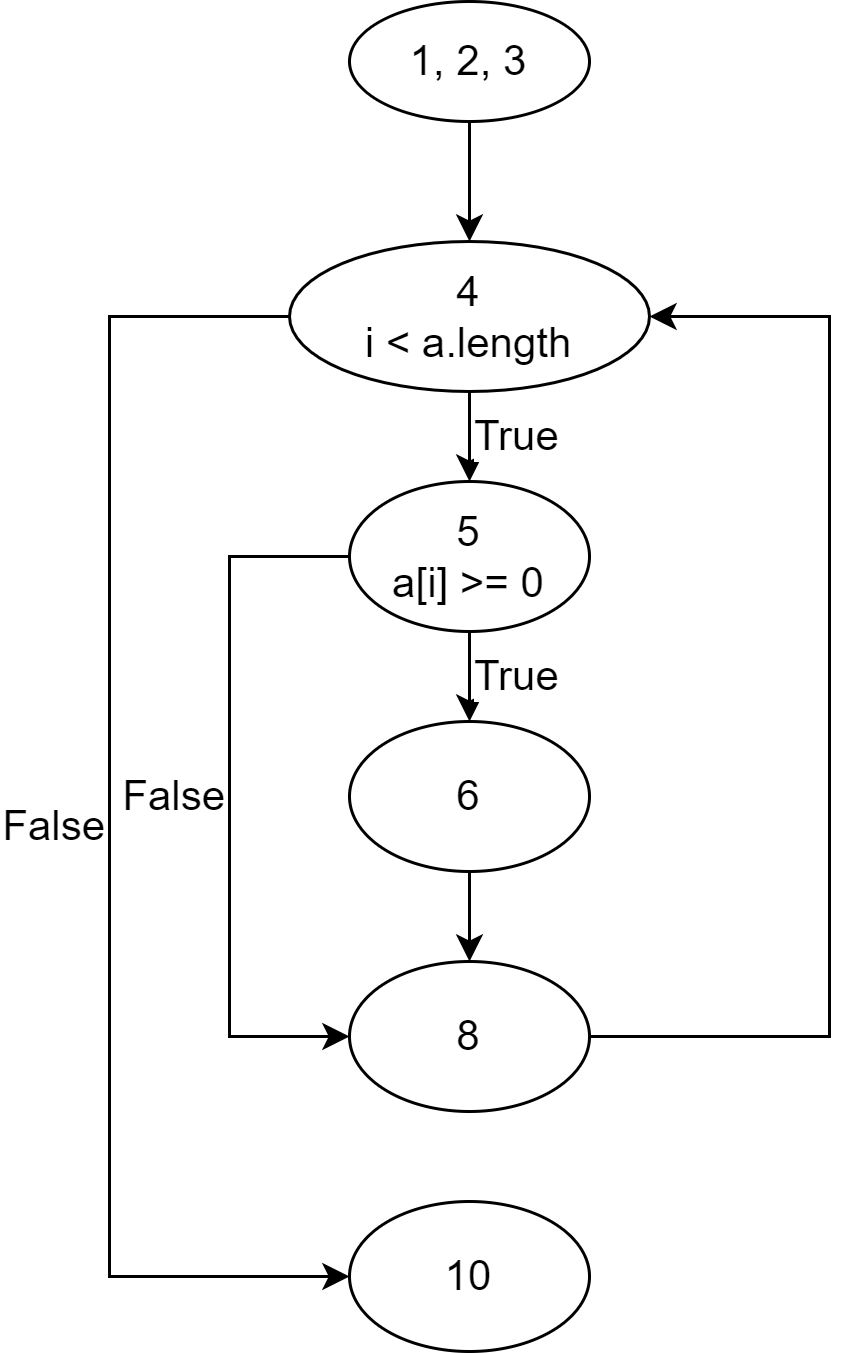
\includegraphics[width=0.4\textwidth]{images/flow-graph-eg.png}
    \caption{Flow graph for the Listing \ref{lst:pos_sum}.}
    \label{fig:flow-graph-eg}
\end{figure}

Intuitively, CC gives us the number of independent paths in the flow graph. There are several ways for calculating CC, $V(G)$. Maybe the simplest one is adding one to the number of closed loops inside the graph. However, a more formal way of calculating CC is given in Eq. \ref{eq:cc-calc}.
\begin{equation}
\label{eq:cc-calc}
    V(G) = E - N + 2
\end{equation}
Here, $E$ is the number of edges, $N$ is the number of nodes. Considering the graph in Figure \ref{fig:flow-graph-eg}, we can calculate CC as $7 - 6 + 2 = 3$. This can also be verified by counting the number of closed loops, which is two, and adding one to it, three.

This result hints us there should be three independent paths in the graph. One can find independent paths by adding a path that is not previously covered by any of the found paths. With this information, we can identify the three independent paths as:

\begin{table}[H]
    \centering
    \renewcommand{\arraystretch}{1.2}
    \caption{Independent paths.}
    \label{tab:independent-paths}
    \begin{tabular}{p{0.1\textwidth}p{0.82\textwidth}}
        \toprule
        \textbf{Path 1} & 1-2-3-4-10\\
        \textbf{Path 2} & 1-2-3-4-5-8-10\\
        \textbf{Path 3} & 1-2-3-4-5-6-8-10\\
        \bottomrule
    \end{tabular}
\end{table}

From these independent paths, we can identify three test cases that force the flow to pass through independent paths. This can be achieved by carefully crafting input variables that satisfy path conditions.

To go through path one, the array should be empty with zero length. After the check of the while condition the flow is directed to the return statement and flow has finished. For path two, the array can have many values but all of them should be negative numbers such as $a = [-5, -1, -2]$. In this path, the flow passes the inside of the if statement and, after a few circulations inside the while statement, is directed to the return statement. For path three, the array can have many integers and some of them must be positive integers such as $a = [-5, 5, 6, -1, 7]$. Here, the flow can travel inside of the if statement as well.

\section{Statement and Branch Coverage}
There are four types of coverage criterion; (1) All-Path Coverage, (2) Statement Coverage, (3) Branch Coverage, and (4) Predicate Coverage. All-Path Coverage covers all of the possible paths and finds all faults. However, some programs even have an infinite number of branches. Therefore, it is not always feasible to perform All-Path Coverage and certainly not in this manual.

Statement Coverage is the weakest one among the others. If a test goes through each statement at least once, we say that the test has 100\% statement coverage. In this chapter's exercises, we will perform Statement Coverage. Writing one test case for each of the independent paths of a program generates 100\% statement coverage.

To achieve full Branch Coverage, we need to select all paths that include at least one branch. The programmer needs to make sure that both true and false outcomes of the conditions are covered at least once.

\section{Exercises}
In this section, there are exercises about CC calculation and test case design. Students should try to solve the exercises without looking to the solutions as much as possible.

\begin{exercise}
    Given the following requirement and its implementation. Test if the given implementation is correct or not by following the below procedure.
    \begin{enumerate}[a),noitemsep]
        \item Draw the flow graph of the function.
        \item Identify the independent paths.
        \item Design the test cases.
        \item Implement the test cases in a class called \lstinline!TotalBillTest!.
    \end{enumerate}

    Keith’s Sheet Music needs a program to implement its music teacher’s discount policy. The program prompts the user to enter the purchase total and indicates whether the purchaser is a teacher. Music teachers receive a 10\% discount on their sheet music purchases unless the purchase total is \$100 or higher. Otherwise, the discount is 12\%. The discount calculation occurs before the addition of the 5\% sales tax.
    
    \begin{lstlisting}
double calculateTotalBill(char customertype, double purchase) {
    double total = purchase;
    if (customertype == 't') {
        if(purchase > 100) {
            total = purchase * 0.91;
        } else {
            total = purchase * 0.88;
        }
    }
    total = total * 1.05;
    return total;
}
    \end{lstlisting}
\end{exercise}

\begin{solution}
    Answer for the item a):
    \begin{figure}[H]
        \centering
        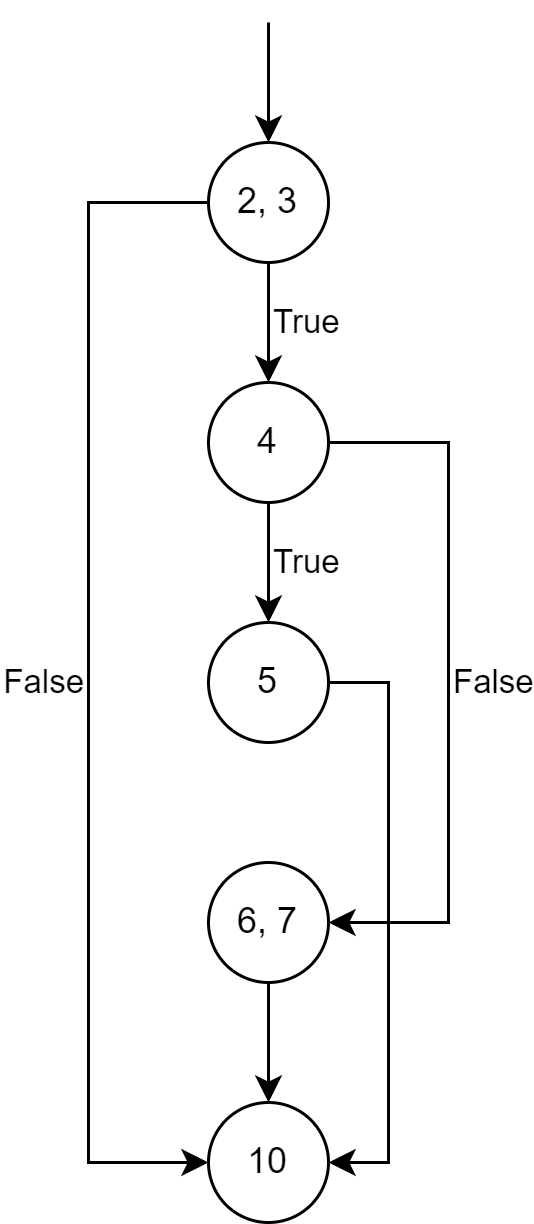
\includegraphics[width=0.3\textwidth]{images/exercise-6a-solution.png}
        \caption{The flow graph of the \lstinline!calculateTotalBill! function.}
        \label{fig:ex6-fg}
    \end{figure}

    Answer for the item b):
    \begin{table}[H]
        \centering
        \renewcommand{\arraystretch}{1.2}
        \caption{Independent paths.}
        \label{tab:ex3-indep-paths}
        \begin{tabularx}{\textwidth}{lX}
            \toprule
             & Independent Path\\
            \midrule
            \textbf{Path 1} & (2,3)-10\\
            \textbf{Path 2} & (2,3)-4-(6,7)-10\\
            \textbf{Path 3} & (2,3)-4-5-10\\
            \bottomrule
        \end{tabularx}
    \end{table}
    
    Answer for the item c):
    
    \begin{table}[H]
        \centering
        \renewcommand{\arraystretch}{1.2}
        \caption{Test cases.}
        \label{tab:ex3-test-cases}
        \begin{adjustbox}{max width=\textwidth}
            \begin{tabular}{lllll}
                \toprule
                 & Independent Path & Test Case & Expected Value & Pass/Fail\\
                \midrule
                \textbf{Path 1} & (2,3)-10 & \lstinline!calculateTotalBill('s', 200.0);! & 210.0 & Pass\\
                \textbf{Path 2} & (2,3)-4-(6,7)-10 & \lstinline!calculateTotalBill('t', 50.0);! & 47.25 & Fail\\
                \textbf{Path 3} & (2,3)-4-5-10 & \lstinline!calculateTotalBill('t', 200.0);! & 184.8 & Pass\\
                \bottomrule
            \end{tabular}
        \end{adjustbox}
    \end{table}
    
    Answer for the item d):
    \begin{lstlisting}
import static org.junit.jupiter.api.Assertions.assertEquals;
import org.junit.jupiter.api.Test;

public class TotalBillTest {

    @Test
    public void testPath1() {
        double result = calculateTotalBill('s', 200.0);
        assertEquals(result, 210.0);
    }
    
    @Test
    public void testPath2() {
        double result = calculateTotalBill('t', 50.0);
        assertEquals(result, 47.25);
    }
    
    @Test
    public void testPath3() {
        double result = calculateTotalBill('t', 200.0);
        assertEquals(result, 184.8);
    }
}
    \end{lstlisting}

\end{solution}

\begin{exercise}
    A hotel offers two types of rooms to their guests. Single rooms are 250TL per day, double rooms are 350TL per day. If a guest chooses a single room and if (s)he prefers to stay more than two days, hotel charges extra 225TL for each day after a single base price of 250TL. If the guest prefers to stay in a double room more than three days, (s)he is supposed to pay 200TL extra for each extra day after a single base price of 350TL.

    \begin{lstlisting}
public class HotelFee {
    public int calculateFee(char type, int day) {
        char roomType = type; 
        int duration = day;
        int price = 3500;
        if (roomType == 'd') {     
            if (duration < 2) {
                price = 350;
            } else if (duration >= 2 && duration <= 10) {
                price = 250 + (duration - 2) * 225;
            }
        } else if (roomType == 's') {
            if(duration < 3) {
                price = duration * 550;
            } else if (duration > 3) {
                price = 250 + (duration - 2) * 225;
            } 
        } 
    return price;
    }
}
    \end{lstlisting}
    
    \begin{enumerate}[a),noitemsep]
        \item Draw the flow graph.
        \item Calculate cyclomatic complexity and independent paths.
        \item Write test cases.
        \item Write the test methods and their results for the test cases in JUnit.
        \item Use a coverage tool (Eclemma) to check the coverage percentage.
    \end{enumerate}
    
    How to Install EclEmma: \url{http://www.eclemma.org/installation.html}\\
    Installation from Update Site

    The update site for EclEmma is \url{http://update.eclemma.org/}. Perform the following steps to install EclEmma from the update site:

    \begin{enumerate}
        \item From your Eclipse menu select Help → Install New Software...
        \item In the Install dialog enter \url{http://update.eclemma.org/} at the Work with field.
    \end{enumerate}
    
    For the usage instructions, follow the link: \url{https://www.eclemma.org/userdoc/index.html}
\end{exercise}

\begin{solution}
    Answer for the item a):
    
    \begin{figure}[H]
        \centering
        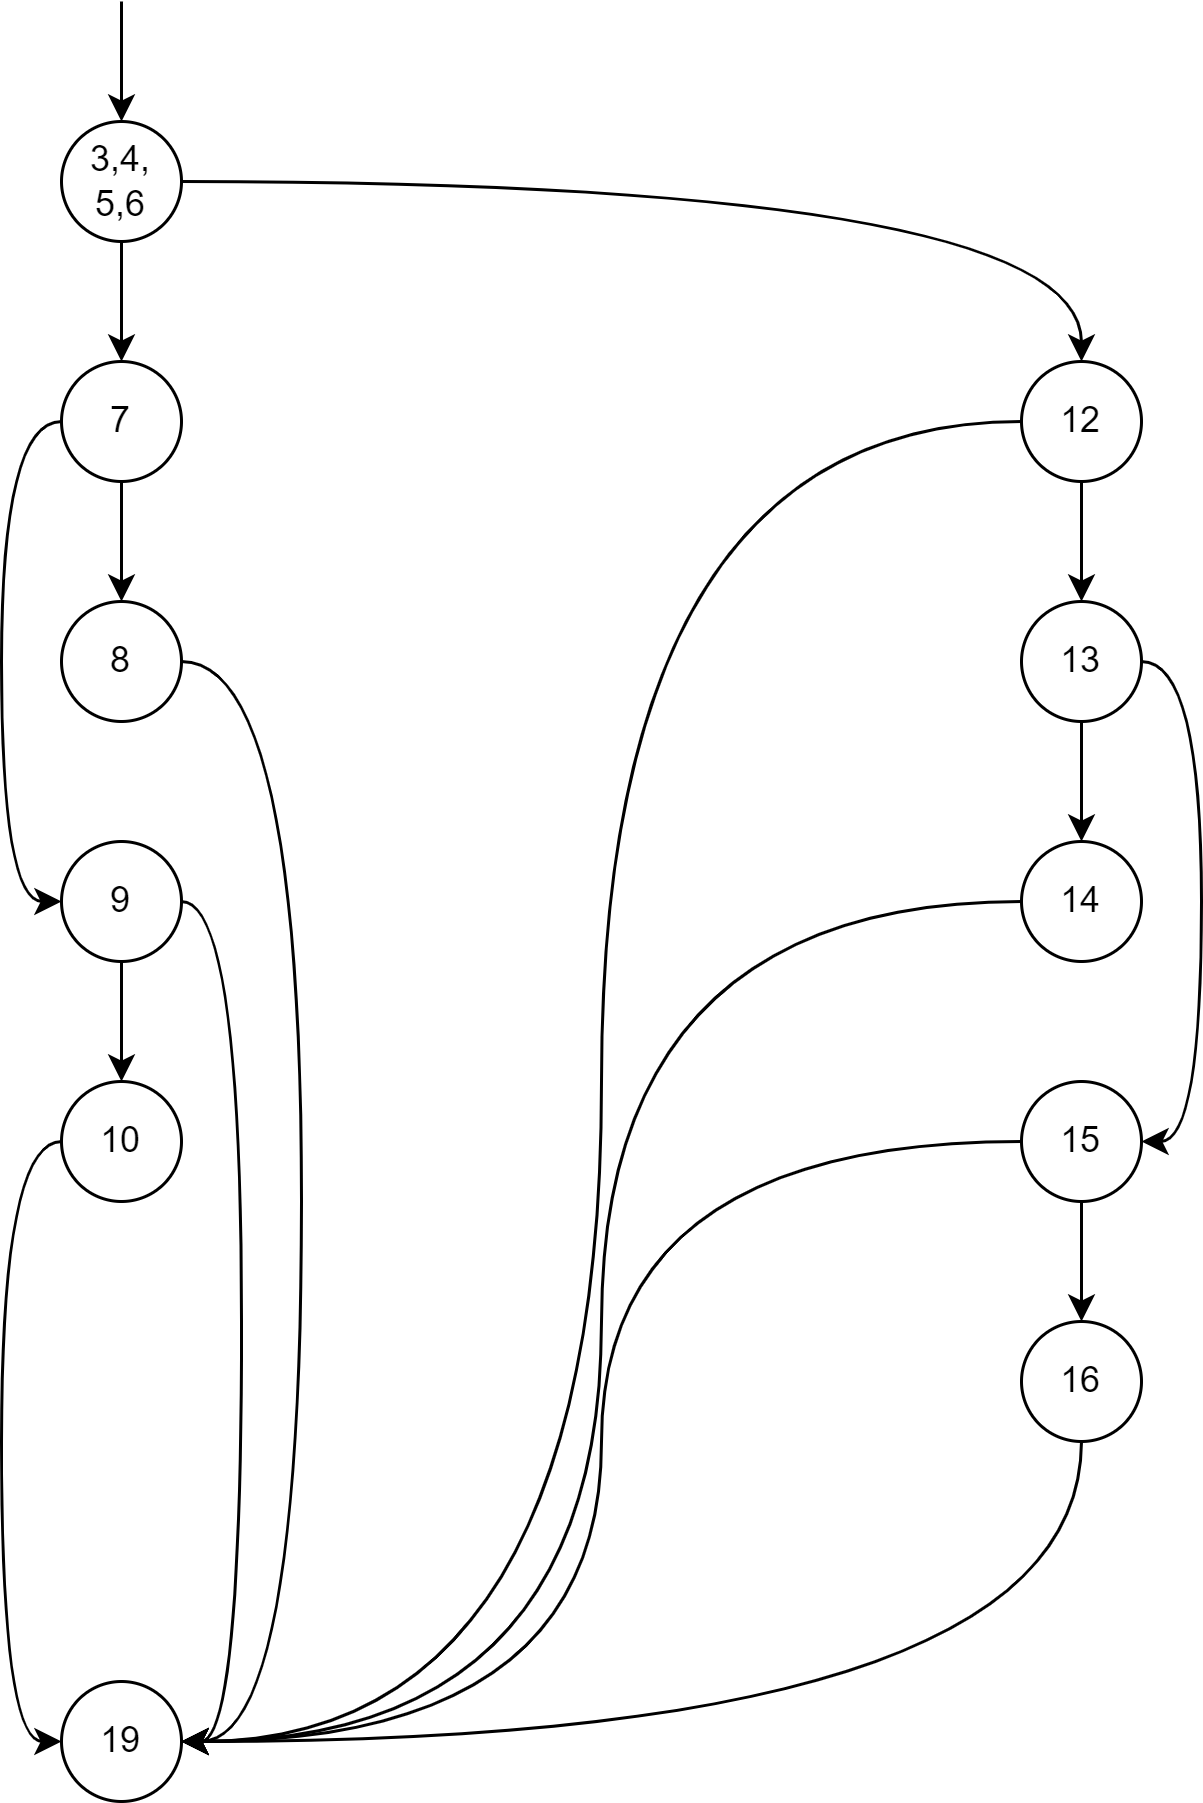
\includegraphics[width=0.5\textwidth]{images/exercise-7a-solution.png}
        \caption{The flow graph of the \lstinline!calculateFee! function.}
        \label{fig:ex7-fg}
    \end{figure}
    
    Answer for the item b):
    
    CC of the graph can be found using the Eq. \ref{eq:cc-calc}; $V(G) = 16 - 11 + 2 = 7$. Therefore, there are seven independent paths in the graph. They are:
    \begin{table}[H]
        \centering
        \renewcommand{\arraystretch}{1.2}
        \caption{Independent paths.}
        \label{tab:ex7-indep-paths}
        \begin{tabularx}{\textwidth}{lX}
            \toprule
             & Independent Path\\
            \midrule
            \textbf{Path 1} & (3,4,5,6)-7-9-19\\
            \textbf{Path 2} & (3,4,5,6)-7-9-10-19\\
            \textbf{Path 3} & (3,4,5,6)-7-8-19\\
            \textbf{Path 4} & (3,4,5,6)-12-19\\
            \textbf{Path 5} & (3,4,5,6)-12-13-15-19\\
            \textbf{Path 6} & (3,4,5,6)-12-13-14-19\\
            \textbf{Path 7} & (3,4,5,6)-12-13-15-16-19\\
            \bottomrule
        \end{tabularx}
    \end{table}
    
    Answer for the item c):
    
    \begin{table}[H]
        \centering
        \renewcommand{\arraystretch}{1.2}
        \caption{Test cases.}
        \label{tab:ex7-test-cases}
        \begin{adjustbox}{max width=\textwidth}
            \begin{tabular}{lllll}
                \toprule
                 & Independent Path & Test Case & Expected Value & Pass/Fail\\
                \midrule
                \textbf{Path 1} & (3,4,5,6)-7-9-19 & \lstinline!calculateFee('d', 15);! & 2750 & Fail\\
                \textbf{Path 2} & (3,4,5,6)-7-9-10-19 & \lstinline!calculateFee('d', 5);! & 750 & Fail\\
                \textbf{Path 3} & (3,4,5,6)-7-8-19 & \lstinline!calculateFee('d', 1);! & 350 & Pass\\
                \textbf{Path 4} & (3,4,5,6)-12-19 & \lstinline!calculateFee('k', 1);! & Error & Fail\\
                \textbf{Path 5} & (3,4,5,6)-12-13-15-19 & \lstinline!calculateFee('s', 3);! & 475 & Fail\\
                \textbf{Path 6} & (3,4,5,6)-12-13-14-19 & \lstinline!calculateFee('s', 2);! & 250 & Fail\\
                \textbf{Path 7} & (3,4,5,6)-12-13-15-16-19 & \lstinline!calculateFee('s', 4);! & 700 & Pass\\
                \bottomrule
            \end{tabular}
        \end{adjustbox}
    \end{table}
    
    Answer for the item d):
    
    \begin{lstlisting}
import static org.junit.jupiter.api.Assertions.assertEquals;
import static org.junit.jupiter.api.Assertions.assertThrows;

import org.junit.jupiter.api.Test;

public class HotelFeeTest {
	
	private final HotelFee hotelFee = new HotelFee();
	
	@Test
	public void testCalculateFeePath1() {
		assertEquals(2750, hotelFee.calculateFee('d', 15));
	}
	
	@Test
	public void testCalculateFeePath2() {
		assertEquals(750, hotelFee.calculateFee('d', 5));
	}
	
	@Test
	public void testCalculateFeePath3() {
		assertEquals(350, hotelFee.calculateFee('d', 1));
	}
	
	@Test
	public void testCalculateFeePath4() {
		assertThrows(UnsupportedOperationException.class, () -> { hotelFee.calculateFee('k', 1); });
	}
	
	@Test
	public void testCalculateFeePath5() {
		assertEquals(475, hotelFee.calculateFee('s', 3));
	}
	
	@Test
	public void testCalculateFeePath6() {
		assertEquals(250, hotelFee.calculateFee('s', 2));
	}
	
	@Test
	public void testCalculateFeePath7() {
		assertEquals(700, hotelFee.calculateFee('s', 4));
	}
}
    \end{lstlisting}
    
    Answer for the item e): 100\% source code coverage should be reported.
\end{solution}

\begin{exercise}
    The Department of Defense identifies soldiers according to some criteria. Only single males whose age is greater than 20 are accepted (martial status: s/S for single, m/M for married, gender: m/M for male, f/F for female). The Department of Defense needs to find a number of candidates that fit this criterion.
    
    \begin{lstlisting}
public class Criteria {
    public int firtsCriteria(int nOfCandid, char[] s, char[] gender, int[] age) {
        int cnt = 1, cntFits = 0;
        while (cnt < nOfCandid) {
            if (s[cnt] == 's' && s[cnt] == 'S' )
                if(gender[cnt] == 'm' || gender[cnt] == 'M')
                    if(age[cnt] > 02)
                        cntFits = cntFits + 1;
            cnt++;
        }	
        return cntFits;
    }
}
    \end{lstlisting}
    
    \begin{enumerate}[a),noitemsep]
        \item Draw the flow graph.
        \item Calculate cyclomatic complexity and independent paths.
        \item Write test cases.
        \item Write the test methods and their results for the test cases in JUnit.
        \item Use a coverage tool (Eclemma) to check the coverage percentage.
    \end{enumerate}
\end{exercise}

\begin{solution}
    Answer for the item a):
    
    \begin{figure}[H]
        \centering
        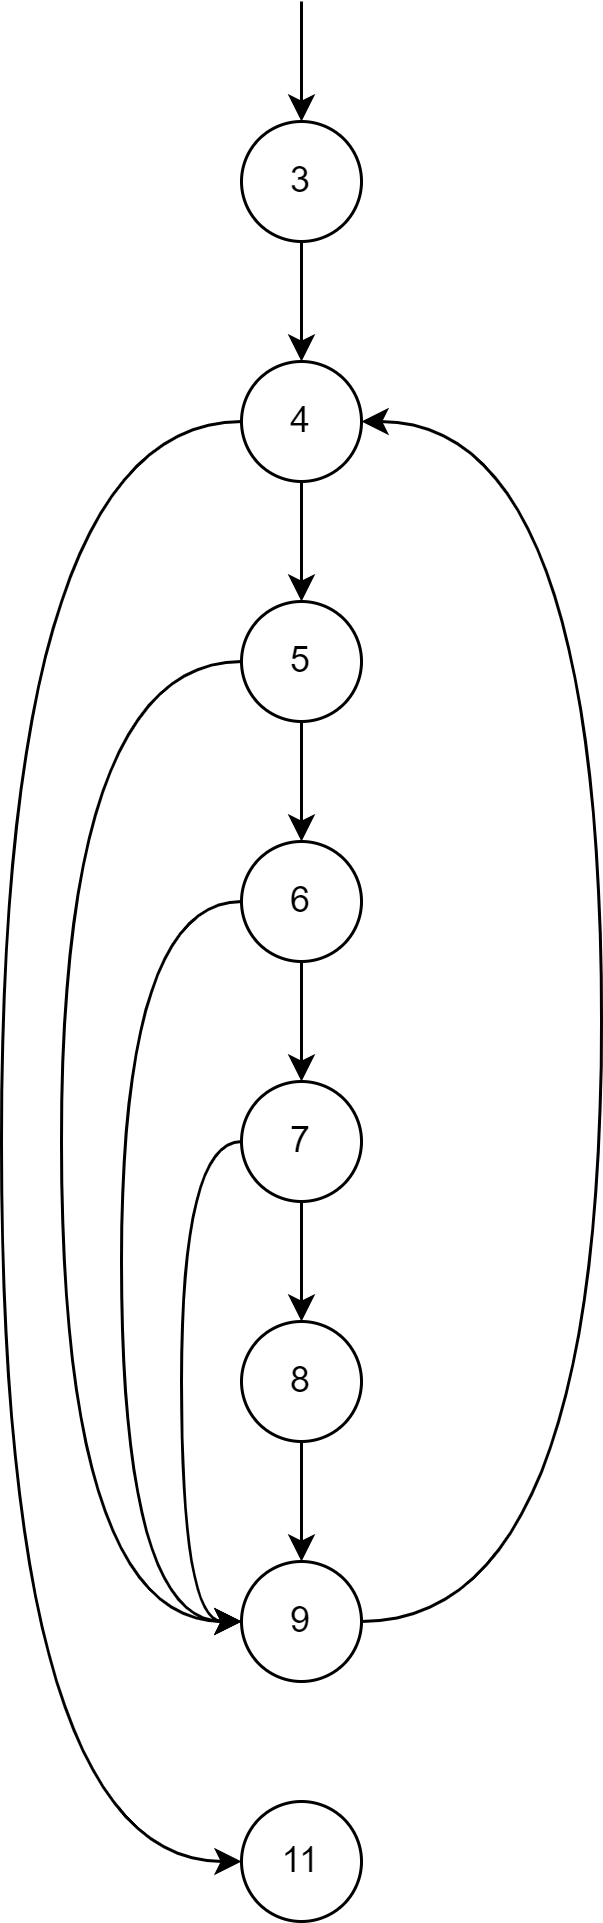
\includegraphics[width=0.25\textwidth]{images/exercise-8a-solution.png}
        \caption{The flow graph of the \lstinline!firstCriteria! function.}
        \label{fig:ex8-fg}
    \end{figure}
    
    Answer for the item b):
    
    CC of the graph can be found using the Eq. \ref{eq:cc-calc}; $V(G) = 11 - 8 + 2 = 5$. Hence, there are five independent paths in the graph. They are:
    \begin{table}[H]
        \centering
        \renewcommand{\arraystretch}{1.2}
        \caption{Independent paths.}
        \label{tab:ex8-indep-paths}
        \begin{tabular}{p{0.1\textwidth}p{0.82\textwidth}}
            \toprule
            \textbf{Path 1} & 3-4-11\\
            \textbf{Path 2} & 3-4-5-9-4-11\\
            \textbf{Path 3} & 3-4-5-6-9-4-11\\
            \textbf{Path 4} & 3-4-5-6-7-9-4-11\\
            \textbf{Path 5} & 3-4-5-6-7-8-9-4-11\\
            \bottomrule
        \end{tabular}
    \end{table}
    
    Answer for the item c):
    
    \begin{table}[H]
        \centering
        \renewcommand{\arraystretch}{1.2}
        \caption{Test cases.}
        \label{tab:e8-test-cases}
        \begin{adjustbox}{max width=\textwidth}
            \begin{tabular}{lllll}
                \toprule
                 & Independent Path & Test Case \lstinline!firtsCriteria(...)! & Expected Value & Pass/Fail\\
                \midrule
                \textbf{Path 1} & 3-4-11 & \lstinline!(1, new char[] {'s'}, new char[] {'m'}, new int[] {22});! & 1 & Fail\\
                \textbf{Path 2} & 3-4-5-9-4-11 & \lstinline!(2, new char[] {'s', 'm'}, new char[] {'m', 'm'}, new int[] {22, 25});! & 1 & Fail\\
                \textbf{Path 3} & 3-4-5-6-9-4-11 & \lstinline!(2, new char[] {'s', 'm'}, new char[] {'f', 'f'}, new int[] {22, 25});! & 0 & Pass\\
                \textbf{Path 4} & 3-4-5-6-7-9-4-11 & \lstinline!(2, new char[] {'s', 's'}, new char[] {'m', 'm'}, new int[] {18, 19});! & 0 & Pass\\
                \textbf{Path 5} & 3-4-5-6-7-8-9-4-11 & \lstinline!(2, new char[] {'s', 's'}, new char[] {'m', 'm'}, new int[] {25, 35});! & 2 & Fail\\
                \bottomrule
            \end{tabular}
        \end{adjustbox}
    \end{table}
    
    Answer for the item d):
    
    \begin{lstlisting}
import static org.junit.jupiter.api.Assertions.assertEquals;

import org.junit.jupiter.api.Test;

public class CriteriaTest {
	
    private final Criteria criteria = new Criteria();
    
    @Test
    public void testPath1() {
        assertEquals(1, criteria.firstCriteria(1, new char[] {'s'}, new char[] {'m'}, new int[] {22}));
    }
    
    @Test
    public void testPath2() {
        assertEquals(1, criteria.firstCriteria(2, new char[] {'s', 'm'}, new char[] {'m', 'm'}, new int[] {22, 25}));
    }
    
    @Test
    public void testPath3() {
        assertEquals(0, criteria.firstCriteria(2, new char[] {'s', 'm'}, new char[] {'f', 'f'}, new int[] {22, 25}));
    }
    
    @Test
    public void testPath4() {
        assertEquals(0, criteria.firstCriteria(2, new char[] {'s', 's'}, new char[] {'m', 'm'}, new int[] {18, 19}));
    }
    
    @Test
    public void testPath5() {
        assertEquals(2, criteria.firstCriteria(2, new char[] {'s', 's'}, new char[] {'m', 'm'}, new int[] {25, 35}));
    }
}
    \end{lstlisting}
    
    Answer for the item e): 60\% source code coverage should be reported.
\end{solution}